\chapter{Design of Experiments}\label{ch:design-experiments}
\initial{C}hapter: ~\ref{ch:research-methodology} documents the design of the hardware and algorithmic implementations of the system that was used.
Section: ~\ref{sec:op-params} shows some of the results obtained in a configuration step and determining the limitations of the unprocessed data.
To evaluate the performance of the designs, several Test suites were planned which exploited the No Line of Sight (NLOS) issue seen in previous sections.
To provide NLOS, rather than systematically occlude an anchor and tag, a person walked a fixed path (see Figure:~\ref{fig:occlude}) at random speeds whilst the data was being recorded.
This was done as to emulate a more realistic environment that the system would be used in.

For tests that had the tag moving two trajectories were outlined.
Table:~\ref{tb:trajs} shows the waypoints of each of the trajectories.
Trajectory one is a quadrilateral whilst trajectory two is a combination of straight-line segments.
In these tests, the tag was moved along the chosen trajectory whilst NLOS occurred randomly due to a person walking.

\begin{figure}[ht!]
    \centering
    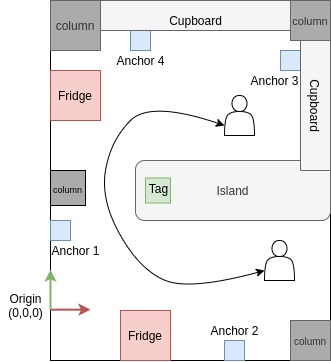
\includegraphics[scale=0.8]{Test_procedure}
    \caption{Path taken by the person to randomly occlude anchors and tag.}
    \label{fig:occlude}
\end{figure}

\begin{table}[ht!]
    \centering
    \begin{tabular}{|c|c|}
        \hline
        & Waypoints $(x,y)$(mm)\\
        \hline
        Trajectory 1 & $\begin{array}{c}
                            (1610, 2080)\\
                            (2111, 2080)\\
                            (1910, 2380)\\
                            (1610, 2580)\\
                            (1610, 2080)
        \end{array}$\\
        \hline
        Trajectory 2 & $\begin{array}{c}
                            (1610, 2080)\\
                            (1710, 2200)\\
                            (1760, 2300)\\
                            (1770, 2500)\\
                            (1840, 2580)\\
                            (1934, 2625)\\
                            (1992, 2595)
        \end{array}$\\
        \hline
    \end{tabular}
    \caption{Trajectories used in the tests for data collection.}
    \label{tb:trajs}
\end{table}
\newpage
\section{Benchmarking and Calibration}\label{sec:benchmarking}
Before testing the system with limitations a benchmark and calibration test was run to record results in an ideal scenario.
This test provided a base that can be used to compare the results of the system operating in non-ideal situations.
Figure: ~\ref{fig:los} shows the results obtained for this benchmarking.
It is seen although the measured position from the tag is slightly noisy, it is well within the $\pm10$cm accuracy quoted by the Pozyx system once the system has started moving and some time has passed.
\begin{figure}[h!]
    \centering
    \begin{subfigure}{0.49\textwidth}
            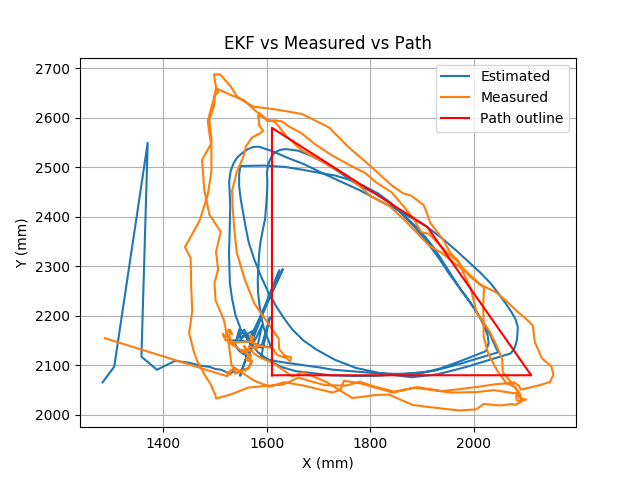
\includegraphics[width=\textwidth]{results/triangle_path_los}
            \caption{Person moving Tag on Trajectory 1.}
    \end{subfigure}
    \begin{subfigure}{0.49\textwidth}
            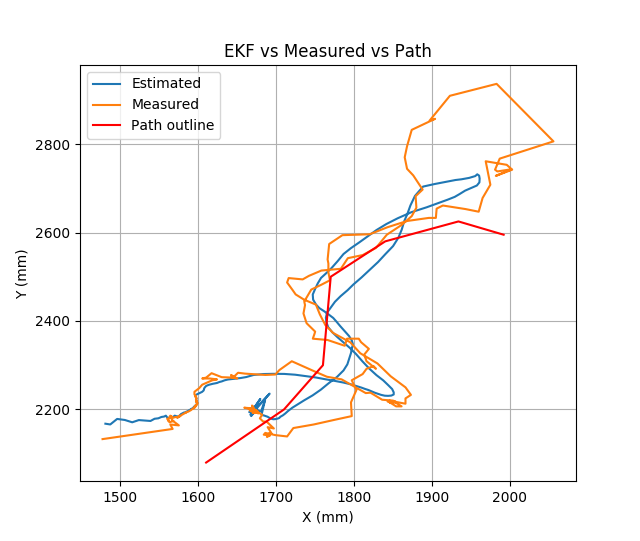
\includegraphics[width=\textwidth]{results/c_path_los}
            \caption{Person moving Tag on Trajectory 2.}
    \end{subfigure}
    \caption{Results for estimation with Line of Sight}
    \label{fig:los}
\end{figure}

\section{Stationary Tags}\label{sec:stationary-tags2}
For these evaluations the designed system was tested with stationary tags, similar to what was done in Section:~\ref{sec:op-params}.
These were carried out to cover the trivial cases where NLOS proved ot be an issue for even a stationary tag.
For the stationary tag tests, the tag was placed at a known point in the workspace and it was introduced to the basic limitations discussed in previous chapters.
The results for the loss of a single anchor was no different than the case recorded previously without the EKF .
However, Figure: ~\ref{fig:stat_anchors} shows the results obtained with the tags located at various positions whilst a person walks randomly in the environment.
In contrast to the previous section, it can be seen the system with the current configuration and EKF is able to withstand NLOS between the anchors and the tag with minimal change in the perceived position.
However, it is evident that the system is now susceptible to a steady-state error which is expected due to the Pozyx's integration with an IMU .
The tag's position will not change drastically and this error will be present as long as the tag is stationary.

\begin{figure}[h!]
    \centering
    \begin{subfigure}{0.49\textwidth}
            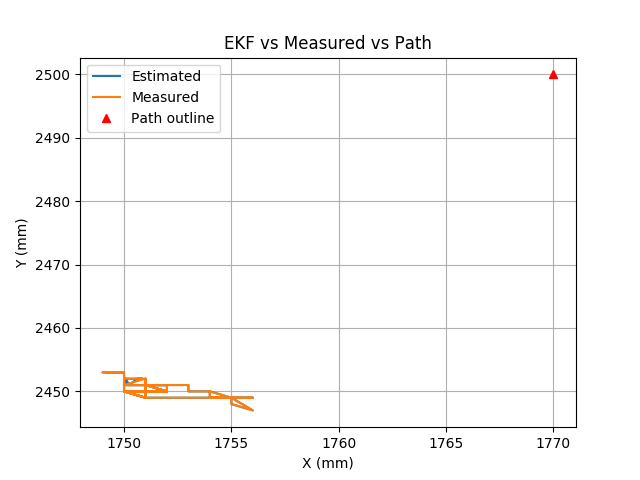
\includegraphics[width=\textwidth]{results/stationary_nlos_(1770,2500)}
            \caption{Result with tag at (1770,2500)}
    \end{subfigure}
    \begin{subfigure}{0.49\textwidth}
            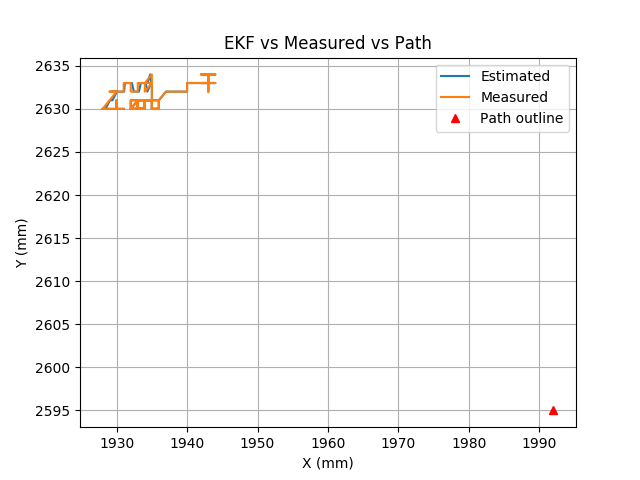
\includegraphics[width=\textwidth]{results/stationary_nlos_(1992,2595)}
            \caption{Result with tag at (1992,2595)}
    \end{subfigure}
    \begin{subfigure}{0.5\textwidth}
            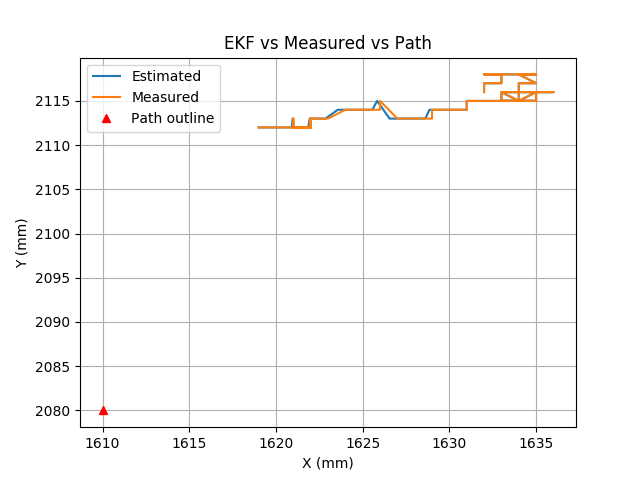
\includegraphics[width=\textwidth]{results/stationary_nlos_origin}
            \caption{Result with tag at (1610,2080)}
    \end{subfigure}
    \caption{Results obtained with No Line of Sight and a Stationary Tag.}
    \label{fig:stat_anchors}
\end{figure}
\newpage

\section{Localisation of a moving target}\label{sec:localisation-of-a-moving-target}
The following experiments would evaluate the designed system while the tag was moving.
This test was done to determine if the processing on the Pozyx tag in addition to an EKF would be able to provide suitable position estimates without the need for any additional measurements or processing.
Figure:~\ref{fig:nlos_ppl} shows the paths recorded for each of these trajectories while the tag was moved by a single person.
It can be seen that as expected the EKF smoothens the supposed trajectory providing a better estimate.
Noteworthy is that using the IMU on the Pozyx tag causes the position to veer slightly on turns.
Additionally, the Pozyx tag was mounted onto a mobile robot that was built to follow a line.
This secondary setup was used to ensure that there was no interference from the person moving the tag and any errors seen would be due to the NLOS caused by the person walking in the environment as seen in Figure: ~\ref{fig:occlude}.
Furthermore, using the mobile robot would indicate if the position estimates would be viable in a fully autonomous scenario.
Figure:~\ref{fig:romi_nlos_1} shows the result obtained while the robot followed Trajectory 2 over two seperate runs.
\begin{figure}[ht!]
    \centering
    \begin{subfigure}{0.7\textwidth}
            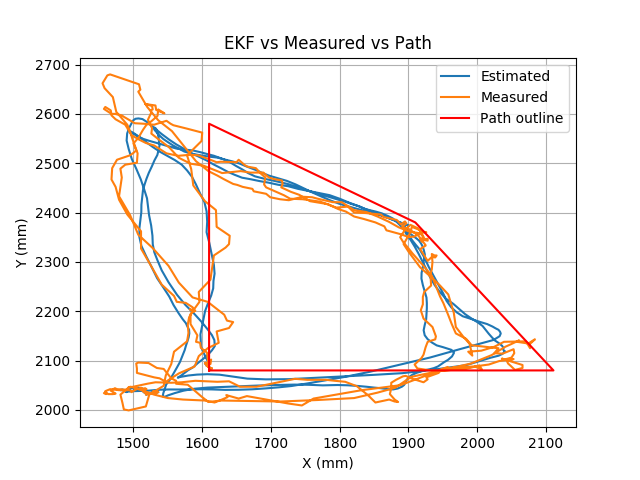
\includegraphics[width=\textwidth]{results/traingle_path_human(nlos)}
            \caption{Movement along Trajectory 1}
    \end{subfigure}
    \begin{subfigure}{0.7\textwidth}
            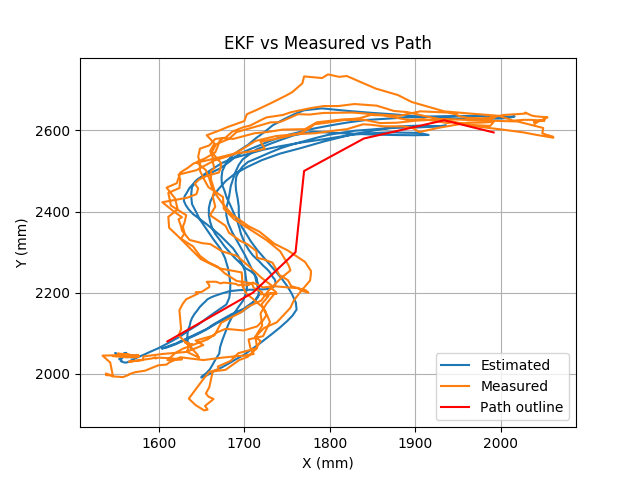
\includegraphics[width=\textwidth]{results/movement_along_c_path_human}
            \caption{Movement along Trajectory 2}
    \end{subfigure}
    \caption{Results obtained with No Line of Sight while the tag is moved by a person.}
    \label{fig:nlos_ppl}
\end{figure}

\begin{figure}[ht!]
    \centering
    \begin{subfigure}{0.7\textwidth}
            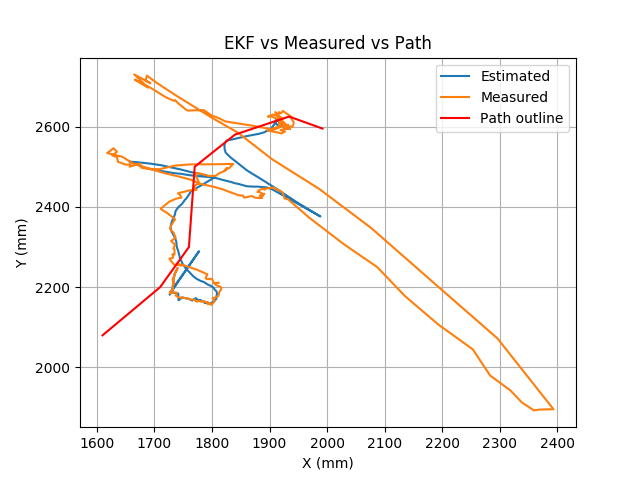
\includegraphics[width=\textwidth]{results/romi_c_path_2}
    \end{subfigure}
    \begin{subfigure}{0.7\textwidth}
            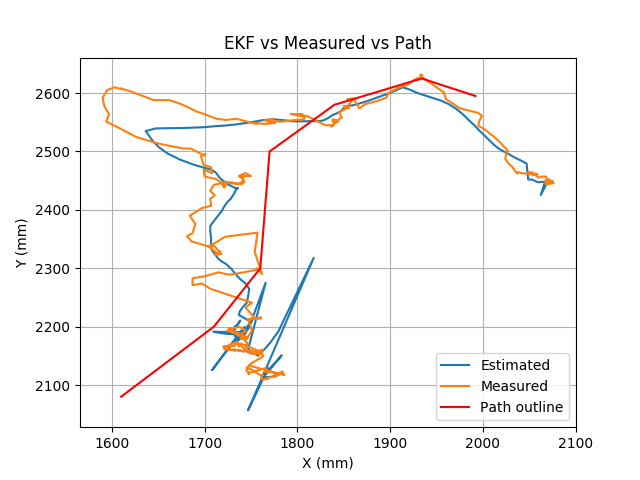
\includegraphics[width=\textwidth]{results/romi_ekf_c_path}
    \end{subfigure}
    \caption{Results obtained with No Line of Sight while the tag was mounted on the mobile robot.}
    \label{fig:romi_nlos_1}
\end{figure}

\section{Improving the Estimates}\label{sec:improving-the-estimates}
In UAV's there are different sensors that provide a multiple measurements for the same state.
As discussed in Section:~\ref{sec:sensor_fusion} it is useful to combine multiple sensor readings in order to improve the overall estimate of the state.
In Section:~\ref{subsec:sensor-fusion} two methods of using the EKF was discussed.
For previous sections of this chapter, the input of the EKF consisted only of the measurements from the Pozyx tag.
In order to compliment the Pozyx measurements, dead reckoning data from the mobile robot was also used as an input into the EKF .
Figure: ~\ref{fig:romi_los} shows the results obtained when the system was run in an ideal situation (Line of Sight).
This was done to once again set a base for comparing the No Line of Sight results.
Figure: ~\ref{fig:romi_nlos_ekf} shows the results obtained from three separate runs of the robot.
The plots show, the actual path taken by the robot, the readings from the Pozyx tag, the readings from the dead reckoning system and the output of the EKF .
\begin{figure}[ht!]
    \centering
    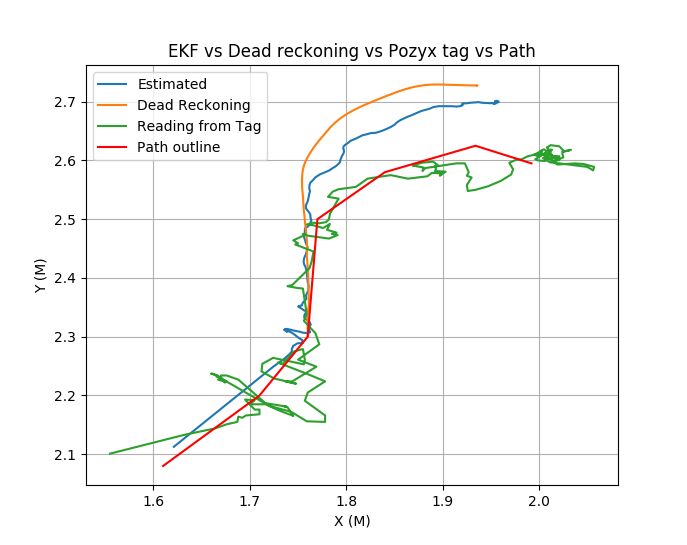
\includegraphics[scale=0.75]{results/romi_ekf_los}
    \caption{Line of Sight estimates from EKF using dead reckoning and Pozyx readings.}
    \label{fig:romi_los}
\end{figure}

\begin{figure}[ht!]
    \centering
    \begin{subfigure}{0.7\textwidth}
            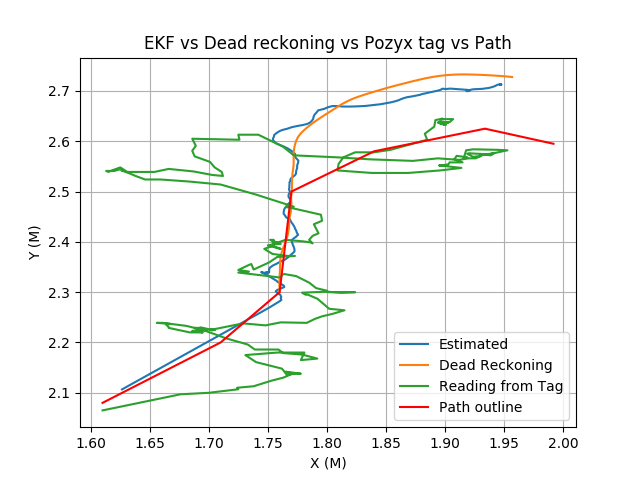
\includegraphics[width=\textwidth]{results/romi_ekf_less_good}
    \end{subfigure}
    \begin{subfigure}{0.7\textwidth}
            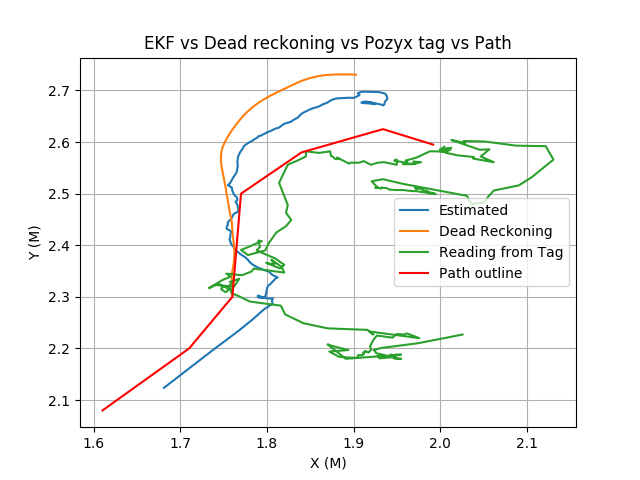
\includegraphics[width=\textwidth]{results/romi_ekf_embed_good_sink_start}
    \end{subfigure}
    \caption{Results obtained with No Line of Sight and EKF estimates using both dead reckoning and Pozyx readings.}
    \label{fig:romi_nlos_ekf}
\end{figure}
\begin{figure}[ht!]\ContinuedFloat
    \centering
    \begin{subfigure}{0.7\textwidth}
            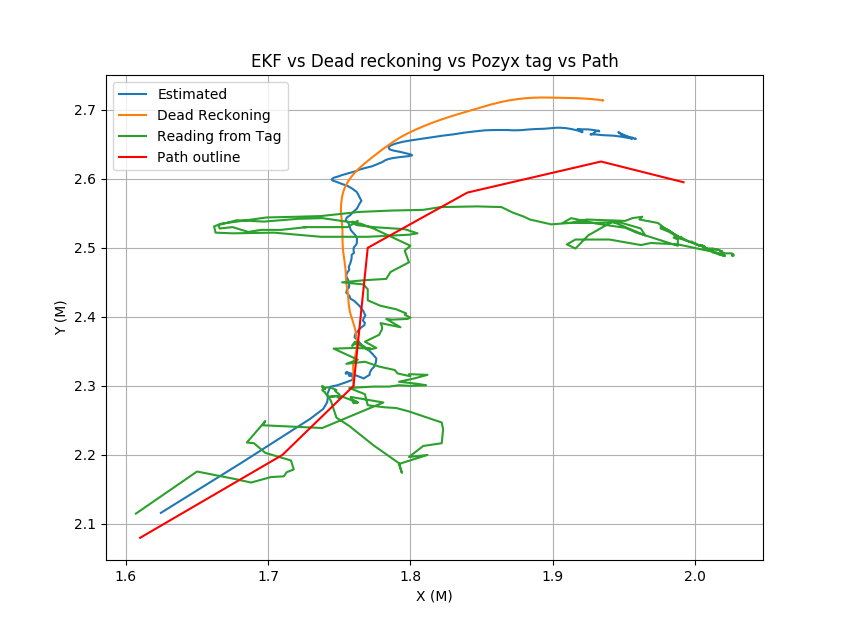
\includegraphics[width=\textwidth]{results/romi_ekf_embed_good}
    \end{subfigure}
    \caption[]{Results obtained with No Line of Sight and EKF estimates using both dead reckoning and Pozyx readings. (cont'd)}
\end{figure}
\newpage
\section{Summary}
This chapter documented the experiments designed and ran in order to evaluate the performance of the Pozyx system for indoor localisation.
These tests were necessary as they addressed the feasibility of using the Pozyx system in UAV's and other forms of autonomous systems.
In the next chapter the results will be discussed providing a qualitative and quantitative analysis of the plots seen in this section.

